% cd /storage/emulated/0/Documents/documents/latex/1920/Grade-10/tests/math-month/ && pdflatex puzzles.tex && termux-open puzzles.pdf

\documentclass[11pt]{article}
\usepackage[letterpaper, portrait, margin=0.5in]{geometry}

\usepackage{xcolor}
\usepackage{anyfontsize}
\usepackage{enumitem}
\usepackage{multicol}
\usepackage{amsmath, makecell}
\usepackage{tabularx} 
\usepackage{gensymb}
\usepackage{wasysym} %for checked symbol 
\usepackage{multirow}
\usepackage{graphicx, tipa}
\usepackage{tikz}
\usetikzlibrary{angles,quotes}
\usepackage{pgfplots} 
\usetikzlibrary{calc}
\pgfplotsset{compat=newest}
\usetikzlibrary{arrows.meta}
\usetikzlibrary{intersections}
\usetikzlibrary{decorations.pathreplacing}
\usepackage{flafter}
%\usepackage{fourier} 
\usepackage{amsmath,amssymb,cancel,units}
\usepackage{microtype} % nicer output 
\usepackage{hfoldsty} % nicer output 
\usepackage{fixltx2e} 
\usepackage{mathptmx}
\usepackage{numprint}
\usepackage[T1]{fontenc}
\usepackage[utf8]{inputenc} 
\usepackage{stackengine} %to define \pesos 
\usepackage{lmodern} %scalable font
\usepackage{booktabs}
\usepackage{array}


\pagenumbering{gobble}
%\linespread{0.9}
\newcommand{\vspce}{\vspace{0.75ex}}

\newcommand{\hspce}{\hspace{0.5em}}

\newcommand{\blank}{\underline{\hspace{2em}}}%{\rule{1em}{0.15ex}}

\newcommand{\arc}[1]{{% 
\setbox9=\hbox{#1}% 
\ooalign{\resizebox{\wd9}{\height}{\texttoptiebar{\phantom{A}}}\cr#1}}}


\newcommand\pesos{\stackengine{-1.4ex}{P}{\stackengine{-1.25ex}{$-$}{$-$}{O}{c}{F}{F}{S}}{O}{c}{F}{T}{S}} 


\renewcommand\theadalign{bc} 

\renewcommand\theadfont{\bfseries} 

\renewcommand\theadgape{\Gape[4pt]} 

\renewcommand\cellgape{\Gape[4pt]} 

\pagenumbering{gobble}

\newcolumntype{Y}{>{\centering\arraybackslash}X} %for tabularx

\newcolumntype{R}{>{\raggedleft\arraybackslash}X} %for tabularx

\newcolumntype{Z}{>{\raggedleft\arraybackslash}X} %for tabularx

\newcolumntype{L}{>{\raggedright\arraybackslash}X} %for tabularx

\newcolumntype{A}[1]{>{\raggedright\arraybackslash}p{#1}} %for longtable LEFT

\newcolumntype{C}[1]{>{\centering\arraybackslash}p{#1}} %for longtable CENTER

\newcolumntype{B}[1]{>{\raggedleft\arraybackslash}p{#1}} %for longtable RIGHT 
 
\renewcommand{\tabularxcolumn}[1]{>{\small}m{#1}}

\newcolumntype{N}[1]{>{\raggedleft}p{#1}} %for tabular left 

\newcolumntype{M}[1]{>{\raggedright\arraybackslash}p{#1}} %for tabular right 

\newcommand{\myaxis}{xticklabels={}, 
yticklabels={}, 
ymin=-10, ymax=10,
xmin=-10, xmax=10,
axis lines = center, 
inner axis line style={Latex-Latex,very thick}, 
grid=both,
minor tick num=4, 
tick align=inside} % grid without labels, origin at the center, 10 units from origin

\newcommand{\axisfive}{xticklabels={}, 
yticklabels={}, 
ymin=-5, ymax=5,
xmin=-5, xmax=5,
axis lines = center, 
inner axis line style={Latex-Latex,very thick}, 
grid=both,
minor tick num=1, 
tick align=inside} % grid with labels, origin at the center, 5 units from origin 

\newcommand \redcheck {{\color{red}\checkmark}}

 

\pagenumbering{gobble}
%\setlength{\extrarowheight}{15pt}


\begin{document} 

\begin{center}
\textbf{Box Challenge}
\end{center} 

\begin{center}
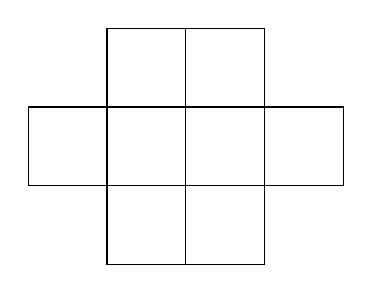
\begin{tikzpicture}

\draw(1,0) rectangle(2,1); 

\draw(0,1) rectangle(-1,2); 

\draw(0,2) rectangle(1,3) rectangle(2,2); 

\draw(0,0) rectangle(1,1) rectangle(2,2) rectangle(3,1);

\end{tikzpicture} 
\end{center} 

Write the digits 1 through 8 in the boxes. No consecutive digits must be placed next to each other, for example: 

\begin{center}
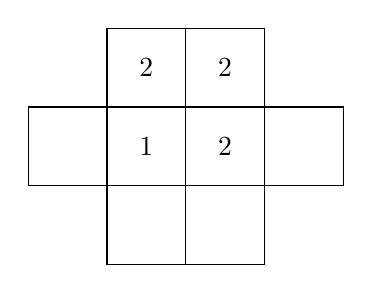
\begin{tikzpicture}

\draw(1,0) rectangle(2,1); 

\draw(0,1) rectangle(-1,2); 

\draw(0,2) rectangle(1,3) rectangle(2,2); 

\draw(0,0) rectangle(1,1) rectangle(2,2) rectangle(3,1);

\node (1) at (0.5, 1.5) {1}; 

\node (2a) at (0.5, 2.5) {2}; 

\node (2b) at (1.5, 2.5) {2}; 

\node (2c) at (1.5, 1.5) {2}; 

\end{tikzpicture} 
\end{center} 

\begin{center}
\textbf{Stick Puzzle}
\end{center} 

Move 6 sticks to form 5 squares. 

%\begin{center}
\begin{tikzpicture}[remember picture,overlay]
\node (stick) at (9,-3){\includegraphics[width=1.5in]{stick.jpg}}; 
\end{tikzpicture} 
%\end{center} 

\newpage 

\begin{center}
\textbf{Coin Puzzle}
\end{center} 

Take six coins and arrange them in a triangle. Your goal is to rearrange the coins into a hexagon in four moves. Each move consists of sliding a single coin to a new location. The new location must be touching at least two other coins at each step. 

%\begin{center}
\begin{tikzpicture}[remember picture,overlay]
\node (coin-start) at (9,-3){\includegraphics[width=1.5in]{coin-start.jpg}}; 
\node (coin-start) at (9,-9){\includegraphics[width=1.5in]{coin-goal.jpg}}; 
\end{tikzpicture} 
%\end{center} 

\end{document} 